\documentclass{standalone}

\usepackage{tikz}
\usepackage{standalone}

\usetikzlibrary{arrows,positioning, decorations.pathreplacing, calc, backgrounds}
\tikzset{
    ncbar angle/.initial=90,
    ncbar/.style={
        to path=(\tikztostart)
        -- ($(\tikztostart)!#1!\pgfkeysvalueof{/tikz/ncbar angle}:(\tikztotarget)$)
        -- ($(\tikztotarget)!($(\tikztostart)!#1!\pgfkeysvalueof{/tikz/ncbar angle}:(\tikztotarget)$)!\pgfkeysvalueof{/tikz/ncbar angle}:(\tikztostart)$)
        -- (\tikztotarget)
    },
    ncbar/.default=0.5cm,
}
\tikzset{square left brace/.style={ncbar=0.5cm}}
\tikzset{square right brace/.style={ncbar=-0.5cm}}

\begin{document}
    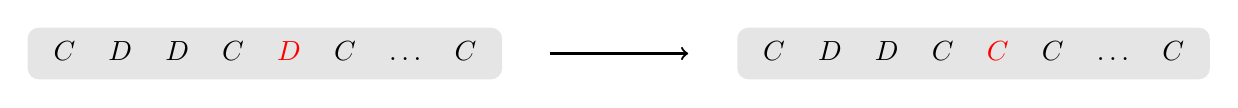
\begin{tikzpicture}
        % \node (n) at (0, 0) {\footnotesize \(N=205\)};
        \node[rectangle, fill=gray!20, rounded corners] (initial_player) at (0, 0) {\begin{tabular}{ccccccccc}
            \(C\) & \(D\) & \(D\) & \(C\) & \textcolor{red}{\(D\)} & \(C\) & \(\dots\) & \(C\) \\
            \end{tabular}};
        \node[rectangle, fill=gray!20, rounded corners] (mutated_player) at (9, 0) {\begin{tabular}{ccccccccc}
                \(C\) & \(D\) & \(D\) & \(C\) & \textcolor{red}{\(C\)} & \(C\) & \(\dots\) & \(C\) \\
                \end{tabular}};

        \node (in) at (3.5, 0) {};
        \node (out) at (5.5, 0) {};
        \draw (in) edge[out=0, in=180, ->, thick] node {} (out);
    \end{tikzpicture}
\end{document}